\section*{2.4 Falsa posición}

Cada par sucesivo de aproximaciones en el método de Bisección incluye una raíz $p$ de la ecuación; esto es, por cada entero positivo $n$ hay una raíz entre $a_n$ y $b_n$. Esto implica que por cada $n$ la iteración del método de Bisección satisface:

\begin{center}
    $|p_n-p|<\frac{1}{2}|a_n-b_n|$,
\end{center}

Lo cual provee una frontera del error fácilmente calculada por las aproximaciones.
La frontera de la raíz no está garantizada para ninguno de los métodos de Newton.

El método de \textbf{Falsa posición} genera aproximaciones e incluye una prueba que asegura que la raíz está delimitada mediante iteraciones sucesivas. 

Primero se elijen las aproximaciones iniciales $p_0$ y $p_1$ con $f(p_0)\cdot f(p_1)<0$ la aproximación $p_2$ es elegida como la intersección de la linea generada de unir $(p_0,f(p_0))$ y $(p_1,f(p_1))$ con el eje x. Para decidir que recta secante usar para calcular $p_3$ se considera $f(p_2)\cdot f(p_1)<0$ o más correctamente $sgnf(p_2)\cdot sgnf(p_1)$.

\begin{itemize}
    \item Si $sgnf(p_2)\cdot sgnf(p_1)<0$ entonces $p_1$ y $p_2$ delimitan a una raíz. Se elige $p_3$ como la intersección de la linea generada de unir $(p_1,f(p_1))$ y $(p_2,f(p_2))$ con el eje x.
    \item Si no, se elige $p_3$ como la intersección de la linea generada de unir $(p_0,f(p_0))$ y $(p_2,f(p_2))$ con el eje x y luego se intercambian los índices en $p_0$ y $p_1$.
\end{itemize}

De manera similar, una vez encontrado $p_3$ el signo de $f(p_3)\cdot f(p_2)$ determina si se usa $p_2$ y $p_3$ o $p_3$ y $p_1$ para calcular $p_4$. En último caso se realiza el reetiquetado de $p_2$ y $p_1$. El reetiquetado asegura que la raíz se encuentra dentro de la frontera mediante iteraciones sucesivas. El proceso es descrito por el algoritmo de \textbf{falsa posición} y la figura \ref{tab:fig5}.

\begin{figure*}[h!]
\centering
  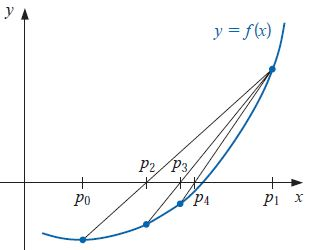
\includegraphics[width=0.6\textwidth]{Falsaposicion.JPG}
\caption{Falsa posición}
\label{tab:fig5}
\end{figure*} 

\begin{tcolorbox}[colback=blue!15!]
\subsubsection*{Falsa posición}
Para encontrar la solución a $f(x)=0$ dada la función continua $f$ en el intervalo $[p_0,p_1]$ donde $f(p_0)$ y $f(p_1)$ tienen signos opuestos:
\\ \\
ENTRADA aproximaciones iniciales $p_0$, $p1$; tolerancia \textit{TOL}; número máximo de iteraciones $N_0$.

SALIDA La solución aproximada \textit{p} o mensaje de falla.

PASO 1 Asigna i=2;

\ \ \ \ \ \ \ \ \ \ \ \ \ \ \ \ \ \ \ \ \ \ \ \ $q_0=f(p_0)$;

\ \ \ \ \ \ \ \ \ \ \ \ \ \ \ \ \ \ \ \ \ \ \ \ $q_1=f(p_1)$.

PASO 2 Mientras $i\leq N_0$ ejecuta los pasos 3-7.

\ \ \ \  PASO 3 Asigna $p=p_1 -q_1(p_1-p_0)/(q_1-q_0) $; (calcula $p_i$)

\ \ \ \  PASO 4 Si $|p-p_0|<TOL$ entonces

\ \ \ \ \ \ \ \ \ \ \ \ \ \ \ \ \ \ SALIDA (p); (proceso completado exitosamente)

\ \ \ \ \ \ \ \ \ \ \ \ \ \ \ \ \ \ ALTO.

\ \ \ \   PASO 5 Asigna $i=i+1$;

\ \ \ \ \ \ \ \ \ \ \ \ \ \ \ \ \ \ \ \ \ \ \ \ \ \ \ \ $q=f(p)$.
    
\ \ \ \   PASO 6 Si $q\cdot q_1<0$ entonces asigna $p_0=p_1$; 

\ \ \ \ \ \ \ \ \ \ \ \ \ \ \ \ \ \ \ \ \ \ \ \ \ \ \ \ \ \ \ \ \ \ \ \ \ \ \ \ \ \ \ \ \ \ \ \ \ \ \ \ \ \ \ \ \ \ \ $q_0=q_1$.

\ \ \ \   PASO 7 Asigna $p_1=p$;

\ \ \ \ \ \ \ \ \ \ \ \ \ \ \ \ \ \ \ \ \ \ \ \ \ \ \ \ $q_1=q$.

PASO 8 SALIDA ('El método fallo después de $N_0$ iteraciones $N_0=$',$N_0$);

\ \ \ \ \ \ \ \ \ \ \ \ \ (El proceso fue exitoso.)

\ \ \ \ \ \ \ \ \ \ \ \ \ ALTO.


\end{tcolorbox}

\subsubsection*{Ejemplo}
Use el método de falsa posición para encontrar la solución a $x=cos x$.

\textbf{Solución}. Se usarán las aproximaciones iniciales $p_0=0.5$ y $p_1=\pi/4$. La tabla \ref{tab:tabla6} muestra el resultado de aplicar el método de falsa posición a $f(x)=cosx-x$.

\begin{table}[h!]
\centering
    \begin{tabular}{||c c||}
    \hline 
    \hline
        \multicolumn{2}{c}{\textbf{Falsa posición}}\tabularnewline
        $n$ & $p_n$      \\
    \hline 
    \hline 
        0 & 0.5 \\
        1 & 0.7853981635 \\
        2 & 0.7363841388 \\
        3 & 0.7390581392 \\
        4 & 0.7390848638 \\
        5 & 0.7390851305 \\
        6 & 0.7390851332 \\
        \hline
        \hline 
    \end{tabular}
\caption{Falsa posición cosx-x}
\label{tab:tabla6} 
\end{table}